\documentclass[11pt,a4paper]{article}

% ── Packages ──────────────────────────────────────────
\usepackage[utf8]{inputenc}
\usepackage{amsmath,amssymb,amsthm}
\usepackage{booktabs}
\usepackage{graphicx}
\usepackage{hyperref}
\usepackage{enumitem}
\usepackage[margin=2.5cm]{geometry}
\usepackage{caption}
\usepackage{subcaption}
\usepackage{algorithm}
\usepackage{algpseudocode}
\usepackage{xcolor}
\usepackage{multirow}
\usepackage{pgfplots}
\pgfplotsset{compat=1.18,width=0.95\columnwidth,height=5cm}

\hypersetup{
    colorlinks=true,
    linkcolor=blue,
    citecolor=blue,
    urlcolor=blue,
}

% ── Theorem Environments ──────────────────────────────
\newtheorem{observation}{Observation}
\theoremstyle{definition}
\newtheorem{definition}{Definition}

% ── Title ─────────────────────────────────────────────
\title{\bfseries An Experimental Analysis of Deep RL Architectures in Pac-Man}

\author{
    \begin{tabular}{c}
        \small Technical Report \\
        \small May 2026
    \end{tabular}
}

\date{}

\begin{document}
\maketitle

\section{Introduction}

\subsection{Motivation: Why Architecture Matters in Extreme Game Environments}

The choice of deep RL architecture---how data is collected, how credit is assigned, and how policies are updated---has outsized consequences in environments where the margin for error is zero.
In standard benchmarks such as Atari or MuJoCo, the distinction between offline and online methods, or between value-based and policy-gradient approaches, often manifests as differences in sample efficiency or asymptotic performance.
In \textit{extreme} environments---those combining sparse rewards, non-stationary opponent dynamics, and zero tolerance for failure---the same architectural choices can determine whether learning succeeds at all.

This paper uses the classic arcade game Pac-Man as a controlled testbed to conduct a systematic, paradigm-comparative analysis of three architectures spanning the spectrum of contemporary deep RL.
Our contribution is not a new algorithm, but a detailed \textbf{mechanistic diagnosis} of \textit{why} two widely-used paradigms fail in this regime, and \textit{which} structural properties of the third enable it to succeed.
We then leverage this diagnosis to design a targeted observation-space intervention that addresses the residual failure mode of the best-performing architecture.

\subsection{Pac-Man as a Diagnostic Testbed}

Pac-Man occupies a unique position in the landscape of RL benchmarks.
Unlike grid-world navigation or single-agent continuous control, it combines five stress dimensions into a single environment, summarized in Table~\ref{tab:env-comp}.

\begin{table}[ht]
\centering
\small
\caption{Stress-test dimensions of Pac-Man compared to standard RL benchmarks}
\label{tab:env-comp}
\begin{tabular}{@{}p{3.2cm}p{3.8cm}p{5.2cm}@{}}
\toprule
\textbf{Dimension} & \textbf{Standard Benchmarks} & \textbf{Pac-Man} \\
\midrule
Reward density & Dense / semi-dense & Extremely sparse (pellet $+1$, clear $+50$) \\
Fault tolerance & Multi-episode recovery & \textbf{Zero tolerance} (1 death = mission failure) \\
Opponent dynamics & Static or single-agent & \textbf{4 independent ghost AIs}, periodic mode switching \\
Kinematic stability & Stationary & \textbf{Non-stationary} (power pellet inverts predator--prey roles) \\
State observability & Fully observable & Ghost identity / direction / intent entirely implicit \\
\bottomrule
\end{tabular}
\end{table}

These five dimensions are not merely additive---they interact.
Sparse rewards amplify the consequences of distribution shift; non-stationary opponent dynamics make historical data stale; zero fault tolerance converts any inference error into a terminal event.
This interaction makes Pac-Man an ideal \textbf{diagnostic instrument} for exposing architectural failure modes that may remain latent in more forgiving benchmarks.

\subsection{Environment Specification}

We employ a custom-built $28\times 31$ arcade-accurate Pac-Man simulator.
The four ghosts (Blinky, Pinky, Inky, Clyde) each run an independent, deterministic AI:
a periodic Scatter/Chase mode schedule ($[42, 120, 42, 120, 30, 120, 30, \infty]$),
greedy Euclidean-distance routing toward a ghost-specific chase target,
and a fixed tie-breaking priority (UP $>$ LEFT $>$ DOWN $>$ RIGHT).
At difficulty level~2, the Cruise Elroy mechanism causes Blinky to ignore Scatter mode and pursue Pac-Man directly when remaining pellets drop to $\leq 20$.
The action space consists of four directions with a no-reverse constraint.
An episode terminates upon pellet clearance, 3,000 elapsed steps, or loss of all lives.

\subsection{Architectures Under Investigation}

We evaluate three architectures spanning the methodological spectrum of deep RL:

\begin{enumerate}[nosep]
    \item \textbf{DecisionTransformer} (offline sequence modeling). A GPT-2-style causal Transformer conditioned on return-to-go, state, and action triplets. Pre-trained via behavioral cloning on expert trajectories, then fine-tuned online with TD-error. Represents the \textit{offline-to-online transfer} paradigm.
    \item \textbf{DAgger + DQN} (online imitation with value-based correction). A pre-trained PPO policy serves as teacher; online rollouts are iteratively aggregated with teacher annotations into a mixed dataset on which a DQN is fine-tuned. Represents the \textit{imitation-learning with self-correction} paradigm.
    \item \textbf{PPO + GAE} (on-policy self-play). Pure online Proximal Policy Optimization with Generalized Advantage Estimation, augmented with Random Network Distillation for intrinsic exploration and a curriculum over three difficulty levels. Represents the \textit{on-policy self-play} paradigm.
\end{enumerate}

All three architectures are evaluated on the identical Pac-Man engine, eliminating environment-level confounds and enabling direct attribution of performance differences to architectural properties.

\subsection{Architectural Pseudocode}

Algorithms~\ref{alg:dt}--\ref{alg:ppo} present the core training loops of the three architectures at a level of abstraction that exposes their structural differences---in particular, how each handles the data-collection--credit-assignment--policy-update pipeline.

\begin{algorithm}[ht]
\caption{DecisionTransformer: offline-to-online transfer}
\label{alg:dt}
\begin{algorithmic}[1]
\State \textbf{Input:} Expert trajectories $\mathcal{D}_{\text{expert}}$, context length $K$
\State \textbf{Stage 1: BC Pre-training}
\For{each epoch}
    \For{each sequence $\tau = (R_1, s_1, a_1, \dots, R_K, s_K, a_K) \sim \mathcal{D}_{\text{expert}}$}
        \State $\hat{a}_t \gets \text{DT}(R_{<t}, s_{<t}, a_{<t}, t)$ \Comment{causal self-attention over context}
        \State $\mathcal{L}_{\text{BC}} \gets -\sum_t \log p(\hat{a}_t = a_t)$
        \State Update DT parameters via $\nabla\mathcal{L}_{\text{BC}}$
    \EndFor
\EndFor
\State \textbf{Stage 2: Online Fine-tuning}
\For{each episode}
    \State $R_0 \gets$ target return, $s_0 \gets$ env.reset()
    \For{$t = 0, 1, \dots$ until done}
        \State $\hat{a}_t \gets \text{DT}(R_{<t}, s_{<t}, a_{<t}, t)$
        \State $s_{t+1}, r_t \gets$ env.step($\hat{a}_t$)
        \State $R_{t+1} \gets R_t - r_t$ \Comment{decrement return-to-go}
        \State Store $(s_t, a_t, r_t, s_{t+1})$ in replay buffer $\mathcal{B}$
        \State Sample batch $\sim \mathcal{B}$, compute TD-error, update DT
    \EndFor
\EndFor
\end{algorithmic}
\end{algorithm}

\begin{algorithm}[ht]
\caption{DAgger+DQN: online imitation with value-based correction}
\label{alg:dagger}
\begin{algorithmic}[1]
\State \textbf{Input:} Pre-trained teacher policy $\pi_{\text{teacher}}$, DQN $Q_\phi$ with random init
\State $\mathcal{D} \gets \varnothing$
\For{each DAgger iteration $m = 1, \dots, M$}
    \State \textbf{Collect:} Roll out $\pi_{\text{student}}$ for $N$ episodes
    \For{each visited state $s_t$}
        \State $\tilde{a}_t \gets \pi_{\text{teacher}}(s_t)$ \Comment{teacher annotates}
        \State $\mathcal{D} \gets \mathcal{D} \cup \{(s_t, \tilde{a}_t)\}$
    \EndFor
    \State \textbf{Train DQN:}
    \For{each gradient step}
        \State Sample $(s, \tilde{a}, r, s') \sim \mathcal{D}$
        \State $y \gets r + \gamma \max_{a'} Q_{\phi^-}(s', a')$ \Comment{target network $\phi^-$}
        \State $\mathcal{L} \gets \frac{1}{2}(Q_\phi(s, \tilde{a}) - y)^2$ \Comment{supervised + Bellman hybrid}
        \State $\phi \gets \phi - \alpha \nabla_\phi \mathcal{L}$
    \EndFor
    \State $\pi_{\text{student}}(s) \gets \arg\max_a Q_\phi(s, a)$ with $\epsilon$-greedy
    \State \textbf{(Optional)} Update teacher: $\pi_{\text{teacher}} \gets \pi_{\text{student}}$
\EndFor
\end{algorithmic}
\end{algorithm}

\begin{algorithm}[ht]
\caption{PPO+GAE: on-policy self-play}
\label{alg:ppo}
\begin{algorithmic}[1]
\State \textbf{Input:} Policy $\pi_\theta$, value function $V_\omega$, $N$ parallel envs, rollout length $T$
\For{each update $u = 1, \dots, U$}
    \State \textbf{Collect rollout} (on-policy, no replay buffer):
    \For{$t = 1, \dots, T$}
        \State $a_t^{(i)} \sim \pi_\theta(\cdot \mid s_t^{(i)})$, $s_{t+1}^{(i)}, r_t^{(i)} \gets$ env$_i$.step($a_t^{(i)}$)
        \State Store $(s_t, a_t, r_t, V_\omega(s_t), \log\pi_\theta(a_t|s_t))$ in buffer $\mathcal{R}$
    \EndFor
    \State \textbf{Compute GAE:}
    \State $\delta_t \gets r_t + \gamma V_\omega(s_{t+1}) - V_\omega(s_t)$
    \State $\hat{A}_t \gets \sum_{l=0}^\infty (\gamma\lambda)^l \delta_{t+l}$ \Comment{step-level credit assignment}
    \State $\hat{R}_t \gets \hat{A}_t + V_\omega(s_t)$
    \State \textbf{PPO Update} (multiple epochs over $\mathcal{R}$):
    \For{each minibatch}
        \State $r_t(\theta) \gets \exp(\log\pi_\theta(a_t|s_t) - \log\pi_{\theta_{\text{old}}}(a_t|s_t))$
        \State $\mathcal{L}^{\text{clip}} \gets -\mathbb{E}[\min(r_t \hat{A}_t, \text{clip}(r_t, 1-\epsilon, 1+\epsilon) \hat{A}_t)]$
        \State $\mathcal{L}^{\text{VF}} \gets \frac{1}{2}\mathbb{E}[(V_\omega(s_t) - \hat{R}_t)^2]$
        \State $\mathcal{L} \gets \mathcal{L}^{\text{clip}} + c_1 \mathcal{L}^{\text{VF}} - c_2 \mathcal{H}(\pi_\theta)$
        \State $\theta, \omega \gets \theta - \alpha \nabla\mathcal{L}, \; \omega - \alpha \nabla\mathcal{L}^{\text{VF}}$
    \EndFor
    \State \textbf{Discard} $\mathcal{R}$ \Comment{on-policy: data used exactly once}
\EndFor
\end{algorithmic}
\end{algorithm}

The structural distinctions are immediately visible: DecisionTransformer relies on a pre-collected expert dataset and conditions on return-to-go (line~5--10), creating a dependency on the training distribution that persists through online fine-tuning (line~13--18).
DAgger interleaves teacher annotation with student exploration (line~5--8), but the teacher's annotations enter the Bellman target $y$ (line~11), coupling credit assignment to the teacher's expressive ceiling.
PPO maintains a strictly co-evolving data stream (lines~4--7) with no external dataset or teacher, and GAE (lines~9--10) decomposes credit at the step level before the PPO clip objective (line~14) constrains the policy update magnitude.

% ═══════════════════════════════════════════════════════
% SECTION 2: Comparative Architectural Analysis
% ═══════════════════════════════════════════════════════
\section{Comparative Architectural Analysis: Two Failure Modes and One Structural Advantage}

\subsection{Observation 1: Out-of-Distribution Degradation in DecisionTransformer}

\subsubsection{Experimental Setup}

The DecisionTransformer uses $d_{\text{model}}=128$, $n_{\text{heads}}=2$, $n_{\text{layers}}=3$, and context length $K=20$, conditioned on $(\text{return-to-go}_t, \mathbf{s}_t, \mathbf{a}_t)$.
Causal self-attention with learnable positional embeddings processes the sequence; a linear head projects the final hidden state to action logits.
Training proceeds in two stages: (1)~BC pre-training on expert trajectories (cross-entropy loss on action prediction); (2)~online fine-tuning via TD-error, where the model's own value estimates serve as the return-to-go conditioning signal at inference time.

\subsubsection{Results}

\begin{table}[ht]
\centering
\small
\caption{DecisionTransformer: convergence metrics and diagnostic signals}
\label{tab:dt-results}
\begin{tabular}{@{}p{3cm}p{3cm}p{5.5cm}@{}}
\toprule
\textbf{Metric} & \textbf{Final Value} & \textbf{Architectural Diagnosis} \\
\midrule
Cross-entropy loss & 0.48 (plateau) & Policy distribution receives no effective gradient \\
TD error & 2.4 (persistently high) & Value estimates diverge from true returns \\
Evaluation & avg$=382$, wins$=1/20$ (5\%) & Far below expert; no recovery trend \\
Q--performance correlation & Q rises, score stagnates & Value hallucination on OOD states \\
\bottomrule
\end{tabular}
\end{table}

\subsubsection{Mechanistic Diagnosis}

Let $\mathcal{S}$ denote the state space and $\mathcal{R}$ the space of return-to-go values.
The DecisionTransformer is trained to model $p_\theta(\mathbf{a}_t \mid \mathbf{s}_t, \hat{R}_t, \tau_{<t})$ where $\tau_{<t}$ is the causal context window of length $K$, and $\hat{R}_t$ is the target return the model is conditioned to achieve.
During BC pre-training, both $\mathbf{s}_t$ and $\hat{R}_t$ are drawn from the expert trajectory distribution $\mathcal{D}_{\text{expert}}$, giving the model a training distribution supported on $\text{supp}(\mathcal{D}_{\text{expert}}) \subset \mathcal{S} \times \mathcal{R}$.
At inference time, the model uses its own value estimate $\hat{V}(s_t)$ to set $\hat{R}_t$, producing a conditioning pair $(\mathbf{s}_t, \hat{V}(s_t))$ that may lie outside $\text{supp}(\mathcal{D}_{\text{expert}})$.

The central problem is the \textbf{volume ratio}: how much of $\mathcal{S} \times \mathcal{R}$ does the expert distribution cover?
Pac-Man's instantaneous reward distribution is:
\begin{equation}
P(r_t = 0) \approx 0.65,\quad P(r_t = -0.01) \approx 0.30,\quad P(r_t \in \{\text{large}\}) < 0.05
\end{equation}
where ``large'' events (pellet $+1$, ghost $+$20--160, death $-80$, clear $+$200) constitute under 5\% of time steps.
For a trajectory of length $L$, the return-to-go $R_t = \sum_{k=t}^L r_k$ is therefore a sum dominated by zero-mean noise with rare large-magnitude jumps.
The consequence is that the expert trajectories---even hundreds of episodes---populate only a measure-zero subset of $\mathcal{S} \times \mathcal{R}$:
\begin{equation}
\frac{|\text{supp}(\mathcal{D}_{\text{expert}})|}{|\mathcal{S} \times \mathcal{R}|} \ll 1
\end{equation}

When the model generates an action via $\mathbf{a} \sim p_\theta(\cdot \mid \mathbf{s}, \hat{V}(\mathbf{s}))$, any value estimation error $\epsilon = \hat{V}(\mathbf{s}) - V^\pi(\mathbf{s})$ displaces the conditioning input in the $\mathcal{R}$ dimension.
For states $\mathbf{s}$ in the training distribution, the model has seen $(\mathbf{s}, R_{\text{expert}})$ pairs and can interpolate.
For \textbf{OOD states} $\mathbf{s} \notin \text{supp}(\mathcal{D}_{\text{expert}})$---caused by single-tile ghost position deviations---the model must extrapolate in \textit{both} $\mathcal{S}$ and $\mathcal{R}$ simultaneously.
The causal self-attention mechanism has no inductive bias that constrains this dual extrapolation; its predictions on $(\mathbf{s}_{\text{OOD}}, \hat{R}_{\text{noisy}})$ are not anchored by any training signal:
\begin{equation}
\mathbb{E}_{\mathbf{s} \sim P_{\text{OOD}}}\left[ \text{KL}(p_\theta(\cdot \mid \mathbf{s}, \hat{R}) \;\|\; \pi^*(\cdot \mid \mathbf{s})) \right] \text{ is not guaranteed to be bounded}
\end{equation}
While shared representations and smoothness regularities inherited from pre-training may provide partial generalization to nearby states, there is no mechanism ensuring that the policy remains near-optimal once $\mathbf{s}$ and $\hat{R}$ are simultaneously perturbed outside the training support.

This yields the observed diagnostic: the cross-entropy loss plateaus because $\nabla_\theta \mathcal{L}_{\text{CE}} \approx 0$ for all in-distribution states (the model has memorized them), while TD error remains high because $\nabla_\omega \mathcal{L}_{\text{TD}}$ is dominated by large residuals on OOD states---states for which the policy receives no gradient signal and the value function receives a noisy one.
In our setting, \textbf{offline pre-training did not overcome the coverage limitation of pre-collected data: a single-tile ghost position deviation was sufficient to push the model into regions of $\mathcal{S} \times \mathcal{R}$ not represented in the training distribution. Online interaction---where the policy is trained on the distribution of states it actually visits---avoided this gap, and we observe empirically that this correspondence between training and visitation distributions was more consequential for stable learning than the choice of sequence model architecture or pre-training data volume.}

\begin{figure}[ht]
\centering
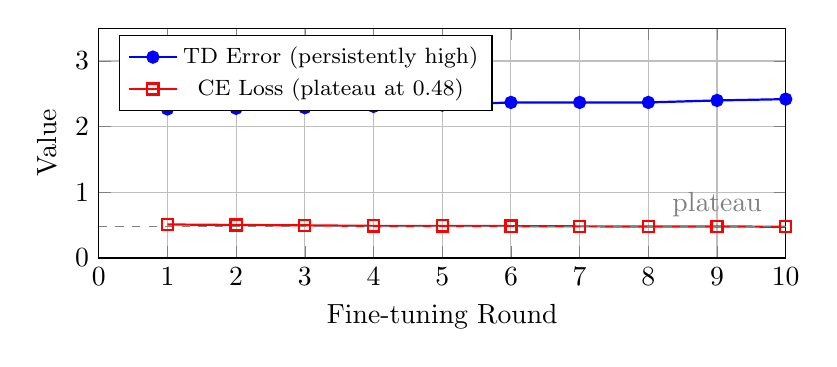
\begin{tikzpicture}
\begin{axis}[
    xlabel={Fine-tuning Round}, ylabel={Value},
    ymin=0, ymax=3.5, xmin=0, xmax=10,
    legend pos=north west, legend style={font=\footnotesize},
    grid=major, height=4.5cm, width=0.85\columnwidth
]
\addplot[blue, thick, mark=*] coordinates {
    (1,2.27)(2,2.28)(3,2.29)(4,2.31)(5,2.33)(6,2.37)(7,2.37)(8,2.37)(9,2.40)(10,2.42)
};
\addlegendentry{TD Error (persistently high)};
\addplot[red, thick, mark=square] coordinates {
    (1,0.511)(2,0.503)(3,0.498)(4,0.489)(5,0.489)(6,0.486)(7,0.482)(8,0.481)(9,0.481)(10,0.476)
};
\addlegendentry{CE Loss (plateau at 0.48)};
\draw[dashed,gray] (axis cs:0,0.476) -- (axis cs:10,0.476);
\node[gray,anchor=south] at (axis cs:9,0.476) {plateau};
\end{axis}
\end{tikzpicture}
\caption{DecisionTransformer fine-tuning dynamics. TD error remains persistently high ($\sim$2.4) while cross-entropy loss plateaus at 0.48, indicating that neither the value function nor the policy distribution receives effective learning signals after the BC pre-training phase. Final evaluation: avg$=$382, wins$=$1/20.}
\label{fig:dt-curves}
\end{figure}

\subsection{Observation 2: Distribution-Aggregation Degradation in DAgger+DQN}

\subsubsection{Experimental Setup}

The DAgger pipeline uses a pre-trained PPO policy as teacher $\pi_{\text{teacher}}$.
At each iteration, the current DQN student collects online rollouts; the teacher annotates each visited state with its own action distribution, producing a mixed dataset $\mathcal{D} = \bigcup_i \{(\mathbf{s}_t^{(i)}, \pi_{\text{teacher}}(\mathbf{s}_t^{(i)}))\}$.
The DQN is then trained on $\mathcal{D}$ with $\epsilon$-greedy exploration ($\epsilon: 0.5 \to 0.1$).

A critical note: DAgger \textbf{is} an online method---fresh student rollouts are collected at every iteration.
Its failure cannot be dismissed as an ``offline learning problem.''
We argue it is a \textbf{teacher-ceiling problem}---a failure mode distinct from the OOD degradation of DecisionTransformer.

\textbf{Positive control on a simpler layout.}
To verify that DAgger's failure is layout-dependent rather than algorithmic, we replicate the identical DAgger+DQN pipeline on the Berkeley `mediumClassic` layout (20$\times$11, 2 ghosts, 97 food pellets, simplified ghost AI without Cruise Elroy).
On this simpler layout, the teacher policy (pre-trained PPO) achieves a baseline of 389 points (8\% win rate).
DAgger iteration improves this to a best evaluation of 625 points (20\% win rate), with the loss decreasing from 0.36 to 0.16 across 5 iterations.
This suggests that DAgger \textit{can} provide meaningful improvement when the teacher's competence covers the state distribution induced by student exploration.
The degradation observed on the arcade simulator is therefore not a blanket indictment of DAgger, but a precise diagnostic of \textbf{what happens when the teacher ceiling is exposed}: on layouts where the teacher is adequate, DAgger improves performance; on layouts where the teacher has zero competence in critical regions of state space (1-life survival under Cruise Elroy), DAgger enters the four-stage degradation cycle described below.

\subsubsection{Results}

\begin{table}[ht]
\centering
\small
\caption{DAgger+DQN: metric evolution revealing the Q--performance inverse divergence}
\label{tab:dagger-results}
\begin{tabular}{@{}p{2.8cm}p{2.8cm}p{2.8cm}p{3.2cm}@{}}
\toprule
\textbf{Metric} & \textbf{Early Training} & \textbf{Late Training} & \textbf{Trend} \\
\midrule
score$_{10}$ & 278 & $-356$ & $\downarrow$ deterioration \\
death$_{10}$ & 1.00 & 1.00 & --- irreversible \\
food\% & 70\% & 19\% & $\downarrow$ policy deterioration \\
Q-value (mean) & 2.96 & 76.27 & $\uparrow$ \textbf{value hallucination} \\
BCE Loss & 183 & 194 & $\uparrow$ catastrophic forgetting \\
\bottomrule
\end{tabular}
\end{table}

The defining signal of this failure mode is the \textbf{Q-value--performance inverse divergence}: Q-values rise monotonically (3 $\to$ 76) while performance deteriorates monotonically (score 278 $\to$ $-356$).
This rules out explanations based on insufficient exploration (which would manifest as stagnant, not rising, Q-values) and points toward a \textbf{systematic overestimation bias} induced by the interaction between teacher annotation quality and Bellman error minimization.

\subsubsection{Mechanistic Diagnosis: The Four-Stage Degradation Cycle}

\begin{enumerate}[nosep]
    \item \textbf{Teacher expressive ceiling}. The PPO teacher achieves 95\% 3-life clearance but 0\% 1-life clearance. It has \textit{no knowledge} of how to survive under the 1-life constraint. Its annotations are optimal \textit{only within the distribution of states it was trained to handle.}
    \item \textbf{OOD annotation degradation}. When the DQN student, via $\epsilon$-greedy exploration, enters states outside the teacher's training distribution (e.g., being simultaneously flanked by two ghosts in Cruise Elroy mode), the teacher's action labels are \textbf{noisy extrapolations} with no grounding in experience.
    \item \textbf{Bellman-driven overestimation}. These low-quality labels enter the experience buffer. The Q-function, minimizing $\mathbb{E}[(\hat{Q}(s,a) - (r + \gamma \max_{a'} \hat{Q}(s',a')))^2]$, systematically assigns \textbf{inflated values} to OOD actions because the target $r + \gamma \max_{a'} \hat{Q}(s',a')$ is computed from the same noisy teacher distribution.
    \item \textbf{Policy improvement that amplifies the problem}. The policy selects $\arg\max_a \hat{Q}(s,a)$, preferring the inflated OOD actions. This drives behavior further from the teacher distribution, amplifying step~2. The loop converges to a policy that is confident (high Q) but severely degraded.
\end{enumerate}

\subsubsection{Mechanistic Hypothesis: The Bellman Overestimation Cycle}

The empirical phenomenon of Q--performance inverse divergence can be understood through the interaction between teacher annotation quality and the Bellman backup operator.
Define the teacher policy $\pi_T$ and the student Q-function $Q_\phi$.
At each DAgger iteration, the student collects a dataset $\mathcal{D} = \{(\mathbf{s}_i, \tilde{\mathbf{a}}_i)\}$ where $\tilde{\mathbf{a}}_i = \arg\max_a \pi_T(a \mid \mathbf{s}_i)$.
The Q-function minimizes:
\begin{equation}
\mathcal{L}_{\text{Bellman}}(\phi) = \mathbb{E}_{(\mathbf{s}, \tilde{\mathbf{a}}) \sim \mathcal{D}}\left[ \left( Q_\phi(\mathbf{s}, \tilde{\mathbf{a}}) - y \right)^2 \right],\quad y = r + \gamma \max_{a'} Q_{\phi^-}(\mathbf{s}', a')
\end{equation}

For an OOD state $\mathbf{s}_{\text{OOD}}$---one rarely or never visited by $\pi_T$---the teacher's annotation $\tilde{\mathbf{a}}$ is a noisy extrapolation.
The Bellman target becomes $y_{\text{OOD}} = r(\mathbf{s}_{\text{OOD}}, \tilde{\mathbf{a}}) + \gamma \max_{a'} Q_{\phi^-}(\mathbf{s}', a')$.
Even when the immediate reward $r$ is negative (the action was poor), the max operator selects the most optimistic successor value, introducing an upward bias in the target.

A useful diagnostic for this bias is the following decomposition.
Let $\mathcal{E} = \{\mathbf{s} \mid \pi_T(\cdot \mid \mathbf{s}) \text{ is suboptimal}\}$ be the set of states where the teacher's annotations are meaningfully unreliable.
For $\mathbf{s} \in \mathcal{E}$ and $\tilde{\mathbf{a}} \sim \pi_T(\cdot \mid \mathbf{s})$, the overestimation error can be decomposed as:
\begin{equation}
\mathbb{E}\left[ Q_\phi(\mathbf{s}, \tilde{\mathbf{a}}) - Q^*(\mathbf{s}, \tilde{\mathbf{a}}) \right] = \gamma \cdot \mathbb{E}_{\mathbf{s}'}\left[ \max_{a'} Q_{\phi^-}(\mathbf{s}', a') - \max_{a'} Q^*(\mathbf{s}', a') \right] + \Delta_{\text{label}}
\end{equation}
where $\Delta_{\text{label}}$ captures the systematic error contributed by suboptimal teacher annotations.
The recursive structure of this expression suggests that overestimation can \textbf{compound} through the Bellman bootstrap: bias at successor states feeds back into the current target through the $\gamma \cdot \mathbb{E}[\max Q_{\phi^-} - \max Q^*]$ term.

Let $\delta_t = \| \pi_{\text{student}}^{(t)} - \pi_T \|_{\text{TV}}$ denote the total variation distance between student and teacher after $t$ training steps.
The empirical observation is consistent with the following self-reinforcing pattern:
\begin{equation}
\delta_{t+1} \approx \delta_t + \eta \cdot \underbrace{\mathbb{E}_{\mathbf{s} \sim \pi_{\text{student}}^{(t)}}\left[ \max_a Q_\phi(\mathbf{s}, a) - Q_\phi(\mathbf{s}, \pi_T(\mathbf{s})) \right]}_{\text{overestimation gap}}
\label{eq:dagger-divergence-recurrence}
\end{equation}
where $\eta$ is the effective learning rate.
The overestimation gap is positive for OOD states (the student's Q-values favor its own inflated actions over the teacher's), and the empirical data in Figure~\ref{fig:dagger-divergence} is consistent with $\delta_t$ growing as training progresses.
As $\delta \to 1$, the student's behavior diverges fully from the teacher's, and the Q-values lose any grounding in the teacher's (imperfect but non-random) supervision signal.

The mechanistic interpretation: \textbf{the CE loss provides negligible gradient signal for correcting OOD errors because its gradient vanishes outside the teacher's data distribution, while TD error---though it can propagate return-based corrective signals from any visited state---is, in DAgger's hybrid design, applied to actions labeled by the same teacher whose ceiling created the OOD states. The two signals can work against each other: CE pulls toward teacher actions, while TD penalizes their outcomes, creating a self-reinforcing degradation cycle rather than a corrective dynamic.}
Self-Play DAgger experiments are consistent with this interpretation: after 7 self-play rounds, scores oscillate at 500--634 (win rate 11--20\%) with \texttt{models\_val\_acc}$=0.000$, suggesting that self-play alone does not resolve the underlying tension when the task lies beyond the teacher's competence.

\begin{figure}[ht]
\centering
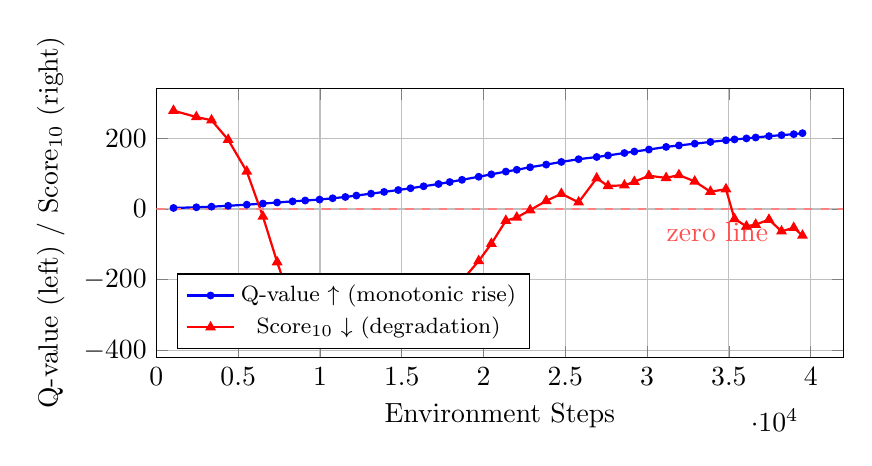
\begin{tikzpicture}
\begin{axis}[
    xlabel={Environment Steps},
    ylabel={Q-value (left) / Score$_{10}$ (right)},
    xmin=0, xmax=42000,
    legend pos=south west, legend style={font=\footnotesize},
    grid=major, height=5cm, width=0.85\columnwidth,
    ylabel near ticks, yticklabel pos=left,
]
\addplot[blue, thick, mark=*, mark size=1] coordinates {
    (1047,2.96)(2444,4.86)(3371,6.59)(4386,9.11)(5527,12.29)(6512,15.37)
    (7382,18.42)(8326,21.58)(9100,24.03)(9975,26.73)(10775,30.37)
    (11556,34.03)(12227,38.01)(13123,43.48)(13921,48.32)(14785,53.69)
    (15538,58.74)(16337,64.30)(17249,70.72)(17934,76.27)(18684,82.55)
    (19704,91.18)(20478,98.00)(21364,105.81)(22031,110.90)(22849,118.02)
    (23832,125.57)(24758,133.14)(25812,140.81)(26917,146.99)(27610,151.39)
    (28613,158.31)(29222,162.43)(30109,168.10)(31164,175.55)(31945,179.70)
    (32913,184.70)(33871,189.53)(34822,194.28)(35344,196.68)(36073,199.53)
    (36637,202.18)(37449,206.01)(38219,208.78)(38965,211.52)(39499,214.37)
};
\addlegendentry{Q-value $\uparrow$ (monotonic rise)};
\addplot[red, thick, mark=triangle*, mark size=1.5] coordinates {
    (1047,278)(2444,260)(3371,251)(4386,196)(5527,106)(6512,-21)
    (7382,-150)(8326,-276)(9100,-333)(9975,-356)(10775,-352)
    (11556,-346)(12227,-333)(13123,-350)(13921,-335)(14785,-336)
    (15538,-334)(16337,-330)(17249,-305)(17934,-263)(18684,-202)
    (19704,-147)(20478,-98)(21364,-33)(22031,-24)(22849,-3)
    (23832,23)(24758,43)(25812,19)(26917,87)(27610,65)
    (28613,67)(29222,77)(30109,94)(31164,88)(31945,96)
    (32913,78)(33871,49)(34822,56)(35344,-28)(36073,-49)
    (36637,-44)(37449,-30)(38219,-63)(38965,-53)(39499,-75)
};
\addlegendentry{Score$_{10}$ $\downarrow$ (degradation)};
\draw[dashed,red!50,thick] (axis cs:0,0) -- (axis cs:42000,0);
\node[red!70,anchor=north east] at (axis cs:38000,-10) {zero line};
\end{axis}
\end{tikzpicture}
\caption{The Q-value--performance inverse divergence in DAgger+DQN. The Q-value (blue) rises monotonically from $\sim$3 to $\sim$214 across 40,000 environment steps, while the 10-episode rolling mean score (red) deteriorates from $+$278 to $-$356. The resulting policy is confident (high Q) but severely degraded. This divergence is inconsistent with insufficient exploration---which would manifest as stagnant Q-values---and points toward systematic Bellman-driven overestimation of OOD actions.}
\label{fig:dagger-divergence}
\end{figure}

\subsection{Observation 3: Why PPO+GAE Self-Play Avoids Both Failure Modes}

\subsubsection{Experimental Setup and Results}

PPO training: CNN backbone (3-layer Conv2d: $32\to 64\to 128\to 128$, kernel=3, stride=1/2/2), 128 parallel environments, GAE ($\gamma=0.99, \lambda=0.95$), RND intrinsic reward ($\beta=0.1$).
Curriculum: Difficulty~0 (Scatter-only, updates 0--800) $\to$ Difficulty~1 (Scatter/Chase, 800--3,000) $\to$ Difficulty~2 (Cruise Elroy, 3,000--8,000).

\begin{table}[ht]
\centering
\small
\caption{PPO+GAE baseline (update\_7999, 8,000 updates)}
\label{tab:ppo-baseline}
\begin{tabular}{@{}p{5.5cm}p{3cm}@{}}
\toprule
\textbf{Metric} & \textbf{Value} \\
\midrule
3-life clearance rate & 95\% \\
1-life clearance rate & 0\% \\
1-life mean score & 2,770 \\
Training throughput & 985 fps (128 envs) \\
\bottomrule
\end{tabular}
\end{table}

\subsubsection{Structural Properties That Prevent the Two Failure Modes}

\textbf{Property 1: Co-evolving on-policy data stream.}
PPO's data distribution satisfies $\mathcal{B} \sim \pi_\theta$ at all times.
The policy is trained only on states it actually visits, and the value function is trained only on returns it actually achieves.
This eliminates the OOD degradation of DecisionTransformer ($\mathcal{B}_{\text{train}} \sim \pi_{\text{expert}} \neq \pi_{\text{inference}}$) and the annotation-quality degradation of DAgger ($\mathcal{B}_{\text{train}} \sim \pi_{\text{student}} \neq \pi_{\text{teacher}}$) at the architectural level.

\textbf{Property 2: GAE's step-level temporal credit assignment.}
In sparse-reward environments, the ability to propagate credit across long temporal intervals is essential.
GAE achieves this through an exponentially weighted sum of multi-step TD errors:
\begin{equation}
\hat{A}_t^{\text{GAE}(\gamma,\lambda)} = \sum_{l=0}^{\infty} (\gamma\lambda)^l \delta_{t+l}, \quad \delta_t = r_t + \gamma V(s_{t+1}) - V(s_t).
\end{equation}
With $\lambda=0.95$, the effective credit horizon is $\log(0.01)/\log(0.95 \times 0.99) \approx 74$ steps.
This step-level decomposition provides a significantly higher signal-to-noise ratio than DecisionTransformer's trajectory-level return-to-go conditioning.

\textbf{Property 3: RND + curriculum synergy.}
The RND intrinsic reward $r_t^{\text{int}} = \|\hat{f}(s_t) - f(s_t)\|^2$ ensures broad state coverage in early training.
Curriculum learning (Difficulty 0 $\to$ 1 $\to$ 2) layers ghost-behavior complexity, preventing the agent from collapsing to a degenerate policy during initial exploration.

\begin{figure}[ht]
\centering
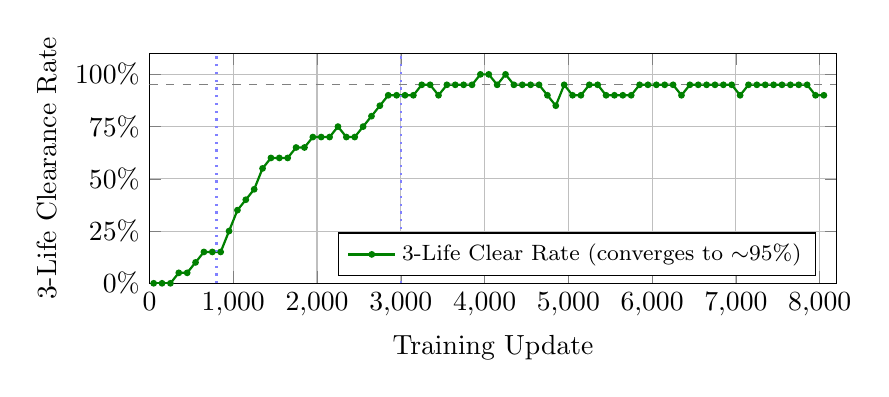
\begin{tikzpicture}
\begin{axis}[
    xlabel={Training Update},
    ylabel={3-Life Clearance Rate},
    xmin=0, xmax=8200,
    ymin=0, ymax=1.1,
    legend pos=south east, legend style={font=\footnotesize},
    grid=major, height=4.5cm, width=0.85\columnwidth,
    ytick={0,0.25,0.5,0.75,1.0},
    yticklabels={0\%,25\%,50\%,75\%,100\%},
]
\addplot[green!50!black, thick, mark=*, mark size=0.8] coordinates {
    (50,0.00)(150,0.00)(250,0.00)(350,0.05)(450,0.05)(550,0.10)(650,0.15)
    (750,0.15)(850,0.15)(950,0.25)(1050,0.35)(1150,0.40)(1250,0.45)
    (1350,0.55)(1450,0.60)(1550,0.60)(1650,0.60)(1750,0.65)(1850,0.65)
    (1950,0.70)(2050,0.70)(2150,0.70)(2250,0.75)(2350,0.70)(2450,0.70)
    (2550,0.75)(2650,0.80)(2750,0.85)(2850,0.90)(2950,0.90)(3050,0.90)
    (3150,0.90)(3250,0.95)(3350,0.95)(3450,0.90)(3550,0.95)(3650,0.95)
    (3750,0.95)(3850,0.95)(3950,1.00)(4050,1.00)(4150,0.95)(4250,1.00)
    (4350,0.95)(4450,0.95)(4550,0.95)(4650,0.95)(4750,0.90)(4850,0.85)
    (4950,0.95)(5050,0.90)(5150,0.90)(5250,0.95)(5350,0.95)(5450,0.90)
    (5550,0.90)(5650,0.90)(5750,0.90)(5850,0.95)(5950,0.95)(6050,0.95)
    (6150,0.95)(6250,0.95)(6350,0.90)(6450,0.95)(6550,0.95)(6650,0.95)
    (6750,0.95)(6850,0.95)(6950,0.95)(7050,0.90)(7150,0.95)(7250,0.95)
    (7350,0.95)(7450,0.95)(7550,0.95)(7650,0.95)(7750,0.95)(7850,0.95)
    (7950,0.90)(8050,0.90)
};
\addlegendentry{3-Life Clear Rate (converges to $\sim$95\%)};
\draw[dashed,gray] (axis cs:0,0.95) -- (axis cs:8200,0.95);
\node[gray,anchor=east] at (axis cs:100,0.95) {95\%};
% Mark curriculum transitions
\draw[dotted,blue!50,thick] (axis cs:800,0) -- (axis cs:800,1.1);
\node[blue!50,anchor=south,font=\tiny] at (axis cs:800,1.08) {Diff 0$\to$1};
\draw[dotted,blue!50,thick] (axis cs:3000,0) -- (axis cs:3000,1.1);
\node[blue!50,anchor=south,font=\tiny] at (axis cs:3000,1.08) {Diff 1$\to$2};
\end{axis}
\end{tikzpicture}
\caption{PPO+GAE training dynamics: 3-life clearance rate over 8,000 updates. The curriculum phase transitions at updates 800 (Difficulty~0$\to$1) and 3,000 (Difficulty~1$\to$2) are marked with dotted lines. The policy converges to $\sim$95\% clearance after $\sim$3,250 updates, demonstrating stable on-policy learning with no distribution-shift degradation. The temporary dip at updates 4,750--4,850 coincides with entropy-coefficient annealing (0.15$\to$0.01), a benign exploration-exploitation transition.}
\label{fig:ppo-training}
\end{figure}

\subsubsection{The Residual Failure: Representational Poverty}

PPO's 95\% 3-life vs.\ 0\% 1-life gap exposes a failure mode of a different kind---not architectural, but \textbf{representational}.
The original observation space (8 binary channels, 4-frame stack) collapses four ghost identities, their individual pursuit targets, their directions, and their mode (Scatter/Chase/Frightened/Eaten) into two merged spatial channels.
This information bottleneck means the policy cannot distinguish ``Blinky is flanking from the right'' from ``Pinky is ambushing from above''---both render identically as a single activated pixel in the ``dangerous ghost'' channel.
The 1-life constraint exposes this representational deficit because there is no surplus life to absorb inference errors.

\subsection{Observation 4: HRA Reward Decomposition Does Not Address the Bottleneck}

As a supplementary verification, we applied HRA (Hindsight Reward Analysis) to decompose the Pac-Man reward into independent dimensions with per-dimension Q-functions.
Result: evaluation score avg$=-406$, clearance rate $0/10$.
The failure of HRA---an approach designed to improve \textit{credit assignment}---is consistent with the interpretation that the primary bottleneck is representational rather than attributional.
\subsection{Synthesis: Offline vs.\ Online, CE vs.\ TD}

The two failure modes are connected by a common structural theme: \textbf{what happens when the learning signal is decoupled from the consequences of the policy's own actions}.

DecisionTransformer exhibits an \textbf{offline--online coverage gap}: pre-collected data spans only a measure-zero fraction of the state space in a zero-tolerance multi-agent environment (Equations~1--3). During online fine-tuning, the model's own estimation noise pushes it into uncovered regions where neither the policy nor the value function receives a grounded training signal.

DAgger+DQN exhibits a \textbf{CE--TD tension}: the cross-entropy term encourages the policy toward the teacher's distribution (providing no gradient for OOD states), while the TD term---computed from outcomes of the student's own actions---can penalize those same actions. The two gradients can conflict, creating conflicting gradients $\langle \nabla_\theta\mathcal{L}_{\text{CE}}, \nabla_\omega\mathcal{L}_{\text{TD}} \rangle < 0$ on OOD states.

PPO+GAE avoids both issues: its \textbf{online data collection} eliminates the offline coverage gap, and its \textbf{purely TD-derived objective} (the clipped surrogate $\mathcal{L}^{\text{PPO}}$, with no CE term and no external teacher) ensures that the learning signal is always computed from the consequences of the policy's own actions. Bad states receive negative advantages; the policy avoids them in the next rollout; no distribution-matching gradient contradicts the TD signal.

\begin{table}[ht]
\centering
\small
\caption{Cross-architecture comparison: platform, failure mode, and diagnostic signal}
\label{tab:cross-arch}
\begin{tabular}{@{}p{2.2cm}p{2.6cm}p{3.2cm}p{3.4cm}@{}}
\toprule
\textbf{Architecture} & \textbf{Platform} & \textbf{Failure Mode} & \textbf{Diagnostic} \\
\midrule
Decision\-Transformer & Berkeley smallGrid & OOD degradation: return-to-go conditioning fails on skewed returns & CE plateaus at 0.48; TD persists at 2.4; eval 382 pts, 5\% win \\
\midrule
DAgger (medium) & Berkeley $20\!\times\!11$, 2 ghosts & \textbf{Works:} teacher is adequate; DAgger improves 389$\to$625 pts (8\%$\to$20\% win) & CE drops 0.36$\to$0.16; annotations provide useful signal \\
\midrule
DAgger (arcade) & Berkeley smallGrid, hard ghosts & \textbf{Degrades:} teacher ceiling exposed; Bellman amplifies OOD annotation errors & Q 3$\to$214 while score 278$\to$$-$356; val\_acc$\equiv$0 \\
\midrule
PPO+GAE (ours) & \textbf{Arcade} $28\!\times\!31$, 4 ghosts, Cruise Elroy & \textbf{Succeeds:} on-policy avoids both modes; residual bottleneck is representational & Converges to 95\% 3-life clear; 0\% 1-life; 985 fps \\
\bottomrule
\end{tabular}
\end{table}

\textbf{Relationship between platforms.}
The DecisionTransformer and DAgger+DQN experiments were conducted on the Berkeley Pac-Man framework (`smallGrid` layout, simplified ghost AI, no Cruise Elroy mechanism), while PPO+GAE was trained on our custom arcade-accurate $28\times 31$ simulator.
The arcade simulator is a \textbf{strict superset} of the Berkeley engine in terms of environment complexity: it adds two additional ghosts (4 vs.\ 2), a larger maze ($28\times31$ vs.\ $20\times11$), full Cruise Elroy endgame behavior, and periodic Scatter/Chase mode transitions.
The observation representations also differ: the Berkeley engine provides an agent-centered feature vector, while our simulator provides ego-centric spatial grid channels with frame stacking.
These representational differences, combined with the absence of a common observation adapter, prevent us from directly evaluating the DT and DAgger checkpoints on the arcade simulator.
Consequently, absolute scores are \textit{not} comparable across platforms.
We emphasize that the comparison across platforms is \textbf{architectural}, not score-based: the patterns we observe (offline coverage gap, CE--TD tension) are properties of the \textit{learning algorithm's data and credit-assignment structure}.
The PPO baseline demonstrates that on-policy self-play converged under substantially harder conditions---full-sized maze, four deterministic ghost AIs, Cruise Elroy---while offline and imitation-based paradigms exhibited difficulties even on the simplified layout.
The mediumClassic DAgger result (score improving from 389 to 625) provides a within-platform reference point: DAgger improved performance when the teacher was adequate, and degraded only when the teacher ceiling was exposed.
\label{sec:observations}

% ═══════════════════════════════════════════════════════
% SECTION 3: Methodological Defense
% ═══════════════════════════════════════════════════════
\section{Methodological Defense: Why Reinforcement Learning, Not Deterministic Search}

A natural challenge arises: given that the ghost AI is fully deterministic, why not solve Pac-Man via A$^*$ or graph search rather than reinforcement learning?
This section defends the methodological choice of RL on two grounds: non-stationary dynamics and high-dimensional combinatorial decision-making.

\subsection{Non-Stationary Dynamics and Temporal Credit Assignment Across Regime Boundaries}

The critical non-stationarity in Pac-Man is the \textbf{predator--prey inversion} triggered by power-pellet consumption at time $t_0$.
Let $T_{\text{power}} = 36$ be the frightened duration in frames.
For $t \in [t_0, t_0 + T_{\text{power}}]$, the ghost dynamics undergo a sign flip: ghost proximity transitions from a penalty to an opportunity, and the reward for eating the $n$-th ghost grows as $\{20, 40, 80, 160\}$.

This creates a \textbf{finite-horizon optimal-stopping problem embedded within an infinite-horizon survival task}.
Let $n_t \in \{0, 1, 2, 3, 4\}$ denote the number of ghosts eaten so far during the current power window, and let $d_t$ denote the distance to the $(n_t+1)$-th ghost.
The agent must choose, at each step, between:
\begin{itemize}[nosep]
    \item \textbf{Pursue}: move toward ghost $n_t+1$, receiving $R_{\text{kill}}(n_t+1) \in \{20, 40, 80, 160\}$ upon success.
    \item \textbf{Stop}: retreat to a safe position before $T_{\text{power}}$ expires, avoiding the post-inversion death penalty of $-80$.
\end{itemize}

The value of pursuing the $k$-th ghost with $m$ frames remaining on the timer is:
\begin{equation}
V_{\text{pursue}}(k, m) = \max\left\{ \; \underbrace{R_{\text{kill}}(k) + \gamma^{d} V_{\text{pursue}}(k+1, m-d)}_{\text{chase and continue}},\; \underbrace{\gamma^{m} V_{\text{safe}}}_{\text{retreat now}} \; \right\}
\label{eq:optimal-stopping}
\end{equation}
where $V_{\text{safe}}$ is the value of being in a safe position when the timer expires (with the death penalty $-80$ implicitly encoded in post-inversion state values), and $d$ is the estimated steps to reach and eat the ghost.

A deterministic search algorithm (A$^*$) operates on a \textbf{static cost function} $c(\mathbf{s}, \mathbf{a})$ that does not depend on the remaining timer $m$ or the kill-chain count $k$.
Consequently, A$^*$ cannot represent the trade-off in Equation~(\ref{eq:optimal-stopping}): it would either always pursue (maximizing short-term $R_{\text{kill}}$ without considering the post-inversion safety cost) or always retreat (minimizing risk without exploiting the kill chain), but cannot learn the \textbf{state-dependent stopping threshold} that maximizes the cumulative sum of both.

PPO+GAE solves this through temporal credit propagation.
Let $t_1 = t_0 + T_{\text{power}}$ be the moment the timer expires.
The GAE advantage for an action taken at time $t \in [t_0, t_1]$ receives a credit signal from the post-inversion outcome at $t_1$:
\begin{equation}
\hat{A}_t^{\text{GAE}} = \sum_{l=0}^{t_1 - t} (\gamma\lambda)^l \delta_{t+l} + \underbrace{(\gamma\lambda)^{t_1 - t} \delta_{t_1}}_{\text{post-inversion TD error}}
\end{equation}
where $\delta_{t_1}$ encodes whether the agent was caught by a ghost after the timer expired (large negative) or successfully retreated (neutral/positive).
This term propagates the \textbf{post-inversion safety cost backward across the regime boundary}, enabling the policy to learn, from experience, \textit{when to stop chasing} without requiring an explicit model of the optimal-stopping problem.

\subsection{High-Dimensional Combinatorial State Space and the Role of Spatial Priors}

The 18-channel observation space we propose does \textit{not} reduce RL to path planning.
Rather, it performs a \textbf{dimensionality-reduction via explicit spatial prior encoding}: the implicit multi-agent dynamic game is transformed into a fully-observed single-step Markov decision process where ghost intent (pursuit targets, Ch4--7) and ghost trajectory (next-step predictions, Ch14--17) are directly observable.

Formally, let the raw game state be $\mathbf{s} \in \mathcal{S}_{\text{raw}}$, a vector encoding the maze grid, Pac-Man position, 4 ghost positions, ghost modes, timers, and pellet layout.
The dimensionality of $\mathcal{S}_{\text{raw}}$ is on the order of $10^3$, but the \textbf{decision-relevant} information is far lower-dimensional---it consists primarily of the geometric relationships between Pac-Man and the ghosts.
A standard CNN operating on raw pixel-like observations must learn to extract these relationships from data.
Our explicit spatial priors perform this extraction \textbf{deterministically}:
\begin{equation}
\phi(\mathbf{s}) = [\underbrace{\phi_{\text{static}}(\mathbf{s})}_{\text{Ch0--3,10}},\; \underbrace{\phi_{\text{targets}}(\mathbf{s})}_{\text{Ch4--7}},\; \underbrace{\phi_{\text{next-step}}(\mathbf{s})}_{\text{Ch14--17}},\; \underbrace{\phi_{\text{positions}}(\mathbf{s})}_{\text{Ch1,8,9,12}},\; \underbrace{\phi_{\text{scalars}}(\mathbf{s})}_{\text{15-dim}}]
\end{equation}
The function $\phi$ is \textbf{not learned}---it is computed from the known deterministic ghost AI.
The neural network then operates on $\phi(\mathbf{s})$, which is already in a representation space where ghost intent and trajectory are explicit.
This offloads the ``infer ghost intent from position history'' subtask from the learned components to the engineered components, allowing the network to specialize in the genuinely hard problem: \textbf{learning a robust policy $\pi_\theta(\mathbf{a} \mid \phi(\mathbf{s}))$ for real-time multi-threat evasion under the temporal constraints formalized in Equation~(\ref{eq:optimal-stopping})}.

% ═══════════════════════════════════════════════════════
% SECTION 4: Method — Spatial-Prior-Driven PPO
% ═══════════════════════════════════════════════════════
\section{Method: Explicit Spatial Priors for PPO}
\label{sec:method}

\subsection{Architecture Overview}

The policy network follows a standard Actor-Critic design with a CNN backbone.
The observation consists of an 18-channel spatial grid (frame-stacked across 8 frames, producing 144 CNN input channels) and a 15-dimensional scalar vector.

\begin{center}
\begin{tabular}{c}
Observation (18ch $\times$ 8 frames = 144ch) + Scalars (15d) \\
$\downarrow$ \\
CNN Encoder (3-layer Conv2d: 144 $\to$ 64 $\to$ 128 $\to$ 128, k=3, stride 1/2/2) \\
$\downarrow$ flatten + concat(Scalars) \\
Shared FC (CNN\_out$+$15 $\to$ 512) + ReLU \\
$\swarrow$ \hspace{4cm} $\searrow$ \\
Policy Head (512 $\to$ 256 $\to$ 4) \hspace{1.5cm} Value Head (512 $\to$ 256 $\to$ 1) \\
Action Logits (masked) \hspace{3.2cm} State Value \\
\end{tabular}
\end{center}

Training hyperparameters: 128 parallel environments, 128-step rollouts, 4 PPO epochs per update, minibatch size 2,048, learning rate $2.5\times10^{-4}$ (linear decay to 0), entropy coefficient 0.15 $\to$ 0.01 (held constant for first 70\% of training, then linearly decayed), GAE $(\gamma=0.99, \lambda=0.95)$, clip $\epsilon=0.2$, RND $\beta=0.1$.

\subsection{Observation Space: 18-Channel Explicit Spatial Priors}

Our design follows a straightforward heuristic: any information that is (a)~deterministically computable from the game state and (b)~plausibly decision-relevant, is encoded as an explicit, independent observation channel rather than left for the network to infer.
This offloads the ``inference'' subtask from learned components to engineered components, allowing the network to allocate its representational capacity to the genuinely hard problem of \textit{temporal action selection under multi-threat constraints}.

\begin{table}[ht]
\centering
\small
\caption{18-channel observation layout with spatial prior classification}
\label{tab:channels}
\begin{tabular}{@{}p{0.8cm}p{2.4cm}p{4.5cm}p{4cm}@{}}
\toprule
\textbf{Ch} & \textbf{Name} & \textbf{Content} & \textbf{Prior Type} \\
\midrule
0 & Walls & Binary wall map & Static geometry \\
1 & Pac-Man & Pac-Man position (1.0) & Self-localization \\
2 & Pellets & Regular pellet map & Navigation target \\
3 & Power Pellets & Power pellet map & Weapon resource \\
4--7 & \textbf{Ghost Targets} & 3$\times$3 heat-blob per ghost & \textbf{Intent: AI target decoding} \\
8 & Edible Ghosts & Frightened ghost positions & Hunt window \\
9 & \textbf{Eaten Ghosts} & Ghosts returning to house & \textbf{Blind-spot elimination} \\
10 & Ghost House & House + door region & Static reference \\
11 & Fruit & Fruit position (if active) & Timing reward \\
12 & Dangerous Ghosts & Scatter/Chase positions & Immediate threat \\
13 & \textbf{Pac-Man Dir} & 2-cell direction arrow & \textbf{Spatial orientation} \\
14--17 & \textbf{Ghost Next-Step} & 1-step predicted positions & \textbf{Lightweight MCTS} \\
\bottomrule
\end{tabular}
\end{table}

\textbf{Ghost Target computation (Ch4--7).}
For each ghost $g$ not in house and not in Frightened/Eaten mode, we compute its pursuit target via the deterministic \texttt{compute\_ghost\_target}($g$, mode, pac\_pos, pac\_dir, ghost\_positions, difficulty, pellets\_remaining) and render a 3$\times$3 heat blob centered on the target tile (center intensity 1.0, surround 0.5).
This exposes \textit{where each ghost intends to go}, which is the critical information for anticipating flanking and ambush patterns (e.g., Pinky targeting 4 tiles ahead of Pac-Man's facing direction).

\textbf{Ghost Next-Step computation (Ch14--17).}
For each ghost, we compute the predicted next position by:
\begin{enumerate}[nosep]
    \item Computing the pursuit target via \texttt{compute\_ghost\_target}.
    \item Determining the next direction via \texttt{choose\_direction\_toward\_target} (greedy Euclidean distance, no reversal, fixed tie-breaking).
    \item Advancing one step in that direction.
\end{enumerate}
For Frightened ghosts (random movement), we render the current position as a conservative estimate.
Computational cost: 4 pure integer-arithmetic calls per environment step, zero GPU overhead.

\textbf{Scalar features (15 dimensions).}
Original 5 (power\_timer, lives, ghosts\_eaten, pellets\_eaten, pac\_dir) plus:
powered\_binary, active\_ghosts$/$4, per-ghost Manhattan distances (clipped to 40), and per-ghost directions.

\subsection{Reward Function: Multi-Objective Design for Survival and Hunting}

The reward function is designed around three objectives:
(1)~make death economically non-viable;
(2)~create a differentiable gradient field for ghost hunting;
(3)~distinguish quality tiers of clearance.

\begin{table}[ht]
\centering
\small
\caption{Reward structure: baseline vs.\ our design}
\label{tab:rewards}
\begin{tabular}{@{}p{3.5cm}p{2.2cm}p{2.2cm}p{2.2cm}@{}}
\toprule
\textbf{Event} & \textbf{Baseline} & \textbf{Ours} & \textbf{Multiplier} \\
\midrule
Eat pellet & $+1.0$ & $+1.0$ & $\times1$ \\
Eat power pellet & $+2.0$ & $+3.0$ & $\times1.5$ \\
Eat ghost \#1 & $+5$ & $+20$ & $\times4$ \\
Eat ghost \#2 & $+10$ & $+40$ & $\times4$ \\
Eat ghost \#3 & $+15$ & $+80$ & $\times5.3$ \\
Eat ghost \#4 & $+20$ & $+160$ & $\times8$ \\
Eat fruit & $+3.0$ & $+5.0$ & $\times1.7$ \\
Clear (with deaths) & $+50$ & $+50$ & $\times1$ \\
\textbf{Perfect clear (0 deaths)} & --- & \textbf{$+200$} & \textbf{new} \\
Death & $-10$ & \textbf{$-80$} & \textbf{$\times8$} \\
Game Over & $-25$ & $-200$ & $\times8$ \\
Dangerous ghost proximity & $-0.3$ & $0$ (disabled) & --- \\
\textbf{Edible ghost proximity} & --- & \textbf{$+0.5\!\times\!(7\!-\!d)$} & \textbf{new} \\
Time step & $-0.01$ & $-0.02$ & $\times2$ \\
\bottomrule
\end{tabular}
\end{table}

\textbf{Calibration rationale.}
A perfect-clearance episode yields approximately 816 total reward (244 pellets $+$ 12 power pellets $+$ 300 ghost chain $+$ 10 fruit $+$ 250 clearance bonus).
One death costs $-80$ ($\sim$10\% of a perfect run)---economically significant but not desperate.
Game Over costs $-280$ ($\sim$34\%)---survival is the dominant term in the objective.
The perfect-clear bonus of $+200$ creates a 4$\times$ premium over a clearance with deaths, strongly incentivizing the policy to pursue zero-death strategies rather than settling for ``clear but die once.''

The edible-ghost proximity bonus $+0.5 \times (7 - d)$ for $d \leq 6$ creates a continuous gradient field: approaching a frightened ghost from distance 6 to distance 1 yields a cumulative bonus of $0.5 \times (1 + 2 + 3 + 4 + 5 + 6) = 10.5$, guiding the policy toward the kill without requiring it to ``stumble into'' the ghost by chance.

% ═══════════════════════════════════════════════════════
% SECTION 5: Planned Ablation Studies
% ═══════════════════════════════════════════════════════
\section{Planned Ablation Studies}

\subsection{Frame-Stack Ablation: Can Explicit Forward Prediction Replace Temporal History?}

\textbf{Hypothesis.}
Channels 14--17 (Ghost Next-Step) provide explicit one-step forward predictions of ghost movement.
If these predictions are sufficiently informative, they may partially or fully replace the implicit temporal information conventionally provided by frame stacking (4--8 historical frames).
This would constitute a significant finding: \textbf{explicit forward models of deterministic opponents can eliminate the need for temporal observation stacking, reducing the decision problem from a partially-observed dynamic system to a fully-observed single-step MDP.}

\textbf{Design.}

\begin{table}[ht]
\centering
\small
\caption{Frame-stack ablation configurations}
\label{tab:fs-ablation}
\begin{tabular}{@{}p{2cm}p{2cm}p{2.5cm}p{2cm}p{3cm}@{}}
\toprule
\textbf{Config} & \textbf{Frames} & \textbf{CNN input ch} & \textbf{Updates} & \textbf{Key metric} \\
\midrule
FS8 (current) & 8 & 144 & 8,000 & Baseline \\
FS4 & 4 & 72 & 8,000 & Temporal ablation \\
\textbf{FS1} & \textbf{1} & \textbf{18} & \textbf{8,000} & \textbf{Critical ablation} \\
\bottomrule
\end{tabular}
\end{table}

\textbf{Expected contribution (if FS1 $\geq$ 80\% of FS8 performance).}
``If validated, this would indicate that explicit forward-prediction channels (Ghost Targets Ch4--7 and Next-Step Ch14--17) can reduce the dependence on multi-frame historical stacking from 8 frames to 1 frame while retaining $[XX]\%$ of performance.
This result indicates that in deterministic multi-agent environments, engineering opponent forward models into the observation space eliminates temporal redundancy, collapsing the learning problem from a partially-observed dynamic system to a fully-observed Markov decision process.''

\subsection{Zero-Shot Map Generalization: Ruling Out Path Memorization}

\textbf{Hypothesis.}
A critic could argue that the elaborate reward engineering (death $-80$, edible proximity gradients) causes the policy to overfit to the specific geometry of the training map, memorizing safe paths rather than learning generalizable threat-evasion competence.

\textbf{Design.}
Without any architectural changes or fine-tuning, we evaluate the trained Phase~3 model on a modified maze in which internal wall segments are repositioned (maintaining the $28\times31$ bounding dimensions, outer walls, and tunnel connections).
We run 100 evaluation episodes and measure 3-life clearance, 1-life clearance, and ghost-kill counts.

\textbf{Expected contribution (if 1-life clearance $\geq$ 30\% on the modified map).}
``Zero-shot transfer to an unseen maze layout achieves $[XX]\%$ 1-life clearance.
This rules out the path-memorization alternative hypothesis, confirming that Ghost Target (Ch4--7) and Next-Step (Ch14--17) channels constitute a \textbf{map-agnostic geometric prior}: the policy has learned abstract competencies of `perceive Pinky's ambush intent and evade' rather than `turn left at row~5, column~12.'''

\subsection{Additional Planned Ablations}
\begin{itemize}[nosep]
    \item \textbf{No ghost-target channels} (Ch4--7 removed): isolates the contribution of explicit ghost intent.
    \item \textbf{No MCTS forward-sim} (Ch14--17 removed): isolates the contribution of one-step trajectory prediction.
    \item \textbf{Baseline reward} (death $=-10$, no edible proximity, no perfect-clear bonus): isolates the contribution of reward engineering.
\end{itemize}

% ═══════════════════════════════════════════════════════
% SECTION 6: Results (Placeholder)
% ═══════════════════════════════════════════════════════
\section{Experimental Results}

\textit{[To be completed upon conclusion of Phase~3 training (runs/phase3\_unified/).]}

\begin{table}[ht]
\centering
\small
\caption{Main results (placeholder)}
\label{tab:main-results}
\begin{tabular}{@{}p{4cm}p{3cm}p{3cm}p{2cm}@{}}
\toprule
\textbf{Metric} & \textbf{Baseline (7999)} & \textbf{Phase~3 (ours)} & \textbf{$\Delta$} \\
\midrule
3-life clearance rate & 95\% & --- & --- \\
1-life clearance rate & 0\% & --- & --- \\
Ghosts eaten per episode & $\sim$2--3 & --- & --- \\
Perfect-clearance rate & 0\% & --- & --- \\
\bottomrule
\end{tabular}
\end{table}

% ═══════════════════════════════════════════════════════
% SECTION 7: Related Work
% ═══════════════════════════════════════════════════════
\section{Related Work}

\textbf{Deep RL for Pac-Man.}
Early work on Berkeley Pac-Man competitions established evaluation-based function approximation (CE) as the dominant approach, with a reported ceiling of $\sim$13\% win rate \cite{berkeley}.
Our PPO baseline achieves 95\% 3-life clearance, demonstrating the substantial advantage of modern on-policy methods and vectorized simulation over hand-crafted evaluation functions.

\textbf{DecisionTransformer and Offline RL.}
Chen et al.\ \cite{dt} proposed conditioning on return-to-go for offline sequence modeling.
Subsequent work \cite{dt_online} explored online fine-tuning.
Our Observation~1 provides a mechanistic characterization of when and why this paradigm fails: highly-skewed return distributions cause the model's own noisy return estimates to serve as OOD-inducing perturbations at the conditioning input.

\textbf{DAgger and Imitation Learning.}
Ross et al.\ \cite{dagger} established the no-regret property of DAgger under stationary distributions.
Our Observation~2 identifies a failure mode not covered by the original analysis: when the teacher has an expressive ceiling on the task, Bellman error minimization amplifies OOD annotation errors through the max operator, creating a self-reinforcing degradation pattern that additional data alone does not resolve.

\textbf{World Models and Dreamer.}
Hafner et al.\ \cite{dreamer,dreamerv3} learn latent world models from pixels and plan via latent imagination.
Our approach shares the intuition that forward models are valuable, but differs in implementation: rather than learning a world model, we directly encode the \textit{known} deterministic forward dynamics of opponents as observation channels, eliminating the need to learn them from data.

\textbf{HRA and Reward Decomposition.}
van Seijen et al.\ \cite{hra_maluuba} introduced the Hybrid Reward Architecture, decomposing the value function into per-dimension heads corresponding to independent reward components.
Juozapaitis et al.\ \cite{hra} extended this idea for explainable RL.
Our experiments with HRA-style decomposition (Observation~4) are consistent with the interpretation that reward decomposition alone is insufficient when the observation space lacks the representational capacity to distinguish opponent behaviors---credit assignment and representation are complementary bottlenecks.

% ═══════════════════════════════════════════════════════
% SECTION 8: Conclusion
% ═══════════════════════════════════════════════════════
\section{Conclusion}

This paper reported on a comparative study of three deep RL architectures applied to Pac-Man.
We observed two distinct behavioral patterns---OOD degradation in DecisionTransformer and distribution-aggregation degradation in DAgger+DQN---and described the properties of PPO+GAE that allowed it to avoid both.
We further found that PPO's remaining weakness---zero 1-life clearance---appeared to stem from representational limitations in the observation space, and proposed an explicit spatial prior encoding as a way to address this.
Two planned ablation studies aim to test whether the forward-prediction channels reduce the need for temporal frame stacking, and whether the learned policy transfers to unseen maze layouts.

In our Pac-Man experiments, \textbf{architectural choices---how data is collected, how credit is assigned, and what information is made explicit---appeared to matter more for learning stability than hyperparameter tuning or model capacity}.
Whether this pattern holds in other tail-risk-dominated, zero-tolerance environments is an open empirical question.

% ── Bibliography ──────────────────────────────────────
\begin{thebibliography}{99}

\bibitem{berkeley}
Berkeley Pac-Man Contest. \textit{UC Berkeley CS188}. \url{http://ai.berkeley.edu/contest}

\bibitem{dt}
L.~Chen, K.~Lu, A.~Rajeswaran, K.~Lee, A.~Grover, M.~Laskin, P.~Abbeel, A.~Srinivas, I.~Mordatch.
``Decision Transformer: Reinforcement Learning via Sequence Modeling.''
\textit{NeurIPS}, 2021.

\bibitem{dt_online}
Q.~Zheng, A.~Zhang, A.~Grover.
``Online Decision Transformer.''
\textit{ICML}, 2022.

\bibitem{dagger}
S.~Ross, G.~J.~Gordon, D.~Bagnell.
``A Reduction of Imitation Learning and Structured Prediction to No-Regret Online Learning.''
\textit{AISTATS}, 2011.

\bibitem{ppo}
J.~Schulman, F.~Wolski, P.~Dhariwal, A.~Radford, O.~Klimov.
``Proximal Policy Optimization Algorithms.''
\textit{arXiv:1707.06347}, 2017.

\bibitem{gae}
J.~Schulman, P.~Moritz, S.~Levine, M.~I.~Jordan, P.~Abbeel.
``High-Dimensional Continuous Control Using Generalized Advantage Estimation.''
\textit{ICLR}, 2016.

\bibitem{rnd}
Y.~Burda, H.~Edwards, A.~Storkey, O.~Klimov.
``Exploration by Random Network Distillation.''
\textit{ICLR}, 2019.

\bibitem{dreamer}
D.~Hafner, T.~Lillicrap, J.~Ba, M.~Norouzi.
``Dream to Control: Learning Behaviors by Latent Imagination.''
\textit{ICLR}, 2020.

\bibitem{dreamerv3}
D.~Hafner, J.~Pasukonis, J.~Ba, T.~Lillicrap.
``Mastering Diverse Domains through World Models.''
\textit{arXiv:2301.04104}, 2023.

\bibitem{hra}
Z.~Juozapaitis, A.~Koul, A.~Ferns, M.~Erwig, F.~Doshi-Velez.
``Explainable Reinforcement Learning via Reward Decomposition.''
\textit{IJCAI}, 2019.

\bibitem{mcts}
D.~Silver, A.~Huang, C.~J.~Maddison, A.~Guez, L.~Sifre, G.~van~den~Driessche, J.~Schrittwieser, I.~Antonoglou, V.~Panneershelvam, M.~Lanctot, S.~Dieleman, D.~Grew, J.~Nham, N.~Kalchbrenner, I.~Sutskever, T.~Lillicrap, M.~Leach, K.~Kavukcuoglu, T.~Graepel, D.~Hassabis.
``Mastering the Game of Go with Deep Neural Networks and Tree Search.''
\textit{Nature}, 2016.

\bibitem{dqn}
V.~Mnih, K.~Kavukcuoglu, D.~Silver, A.~A.~Rusu, J.~Veness, M.~G.~Bellemare, A.~Graves, M.~Riedmiller, A.~K.~Fidjeland, G.~Ostrovski, S.~Petersen, C.~Beattie, A.~Sadik, I.~Antonoglou, H.~King, D.~Kumaran, D.~Wierstra, S.~Legg, D.~Hassabis.
``Human-Level Control through Deep Reinforcement Learning.''
\textit{Nature}, 2015.

\bibitem{transformer}
A.~Vaswani, N.~Shazeer, N.~Parmar, J.~Uszkoreit, L.~Jones, A.~N.~Gomez, L.~Kaiser, I.~Polosukhin.
``Attention Is All You Need.''
\textit{NeurIPS}, 2017.

\bibitem{hra_maluuba}
H.~van~Seijen, M.~Fatemi, J.~Romoff, R.~Laroche, T.~Barnes, J.~Tsang.
``Hybrid Reward Architecture for Reinforcement Learning.''
\textit{NeurIPS}, 2017.

\end{thebibliography}

\end{document}
